As mentioned in the introduction (see Section~\ref{Introduction}), understanding whether neural network models are similar is crucial in many areas of research and application.
This chapter is primarily based on the work by Klabunde et al.~\cite{klabunde_similarity_2024}, with additional references cited where appropriate.
Since there are various perspectives on what it means for models to be similar, we focus on two central and state-of-the-art viewpoints, illustrated in Figure~\ref{fig:SimilarityOfNN}. These are:
\begin{itemize}
    \item Representational similarity, and
    \item Functional similarity
\end{itemize}

We examine the key perspectives of \textit{representational similarity measures} and \textit{functional similarity measures} in more detail in Sections~\ref{RMS} and~\ref{FMS}, respectively.
%Similarity metrics have been widely studied, especially in relation to the invariance properties of neural networks~\cite{ding_grounding_2021, kornblith_similarity_2019}.



\begin{figure}[h]
    \centering
    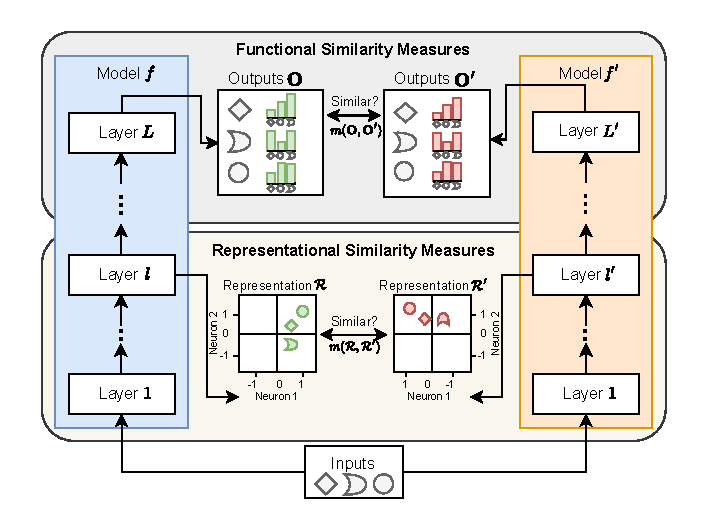
\includegraphics[width=\linewidth]{Abschlussarbeit/Pictures/Similarity90Deg.drawio.pdf}
    \caption{Visualization of representational and functional similarity \cite{klabunde_similarity_2024}.}
    \label{fig:SimilarityOfNN}
\end{figure}

